%! TeX program = lualatex

\documentclass[12pt]{article}

\usepackage{cmap}

\usepackage[english, russian]{babel}

\usepackage{microtype}

\usepackage{float}
\usepackage{fontspec}
\usepackage[pdfborder={0 0 0}]{hyperref}

\usepackage{lipsum}

\usepackage{enumitem}
% \usepackage{libertinus}

% \setmainfont{Ubuntu}

\setmainfont{TimesNewerRoman}[
  Extension = .otf,
  Path = /nix/store/ihdqrn4p54awd89vrday9k53s8i47bbv-times-newer-roman-unstable-2018-09-11/share/fonts/opentype/,
  UprightFont = *-Regular,
  BoldFont = *-Bold
]
\setmonofont{Source Code Pro}

\newcommand{\icon}[1]{\fontspec{UbuntuNerdFont}[Extension = .ttf, 
  Path = /nix/store/h721jafy2n74x4k5p0hxbz722h0rncmx-nerd-fonts-ubuntu-3.3.0+0.83/share/fonts/truetype/NerdFonts/Ubuntu/,
  UprightFont = *-Regular, 
BoldFont = *-Bold] #1}

\usepackage{graphicx}
\usepackage{multicol}
\usepackage{xcolor} % Цвета

\usepackage{fontawesome5} % Для иконок

\usepackage[left=2.0cm, right=2.0cm, top=1.0cm, bottom=1.0cm, includeheadfoot]{geometry}

% \usepackage[mocha, textcolor=true, pagecolor=true]{catppuccinpalette}
\usepackage[latte, textcolor=true, pagecolor=true]{catppuccinpalette}

% \usepackage[\jobname,styleAll]{catppuccinpalet}

\usepackage{amsmath}
\usepackage{amsfonts}
\usepackage{amssymb}
\usepackage{listings}

% NOTE: включить при компиляции
% \usepackage{setspace}
% \onehalfspacing

\usepackage{fancyhdr}

\fancyhf{}

% \renewcommand{\sectionmark}[1]{\markboth{#1}}{\rightmark}
\renewcommand{\subsectionmark}[1]{\markright{#1}{\leftmark}}
\renewcommand{\sectionmark}[1]{\markright{#1}{\leftmark}}

% Настройка колонтитулов
\fancyhead[RO]{\rightmark}  % section (справа)
\fancyhead[LO]{\leftmark}   % subsection (слева)

\fancyfoot[L]{\hspace{8pt} \rule{\textwidth}{0.4pt}}
\fancyfoot[R]{\LARGE{\thepage}}
\fancyfoot[C]{}

\newcommand{\lablogo}
{
\begin{center}
    \huge{\textbf{Лабораторная работа №3}} \\
\end{center}
}

\newcommand{\colorURL}[1]{\textcolor{CtpBlue}{#1}}
\newcommand{\colorGIT}[1]{\textcolor{CtpGreen}{#1}}

\lstdefinestyle{csharp_catppuccin}{
    language={[Sharp]C},
    breaklines=true,
    literate={*}{{\char42}}1
               {-}{{\char45}}1
               {\ }{{\copyablespace}}1,
               % {``}{{``}}1
               % {''}{{''}}1
               % {“}{{``}}1
               % {”}{{''}}1
               % {"}{{\textquotedbl}}1,
    inputencoding=utf8,
    extendedchars=true,
    captionpos=b,
    frame=tb,
    texcl=true,
    keepspaces=true,
    columns=fullflexible,
    showstringspaces=false,
    breakatwhitespace=true,
    morecomment=[l]{//}, %use comment-line-style!
    morecomment=[s]{/*}{*/}, %for multiline comments
    stringstyle={\color{CtpGreen}},
    moredelim=[s][\color{CtpGreen}]{"""}{"""},
    % moredelim=[s][\color{CtpGreen}]{"}{"},
    commentstyle={\color{CtpOverlay1}},
    basicstyle={\scriptsize\color{CtpText}\ttfamily},
    keywordstyle={\color{CtpMauve}},         % Основные ключевые слова
    keywordstyle=[2]{\color{CtpMauve}},      % Модификаторы доступа
    keywordstyle=[3]{\color{CtpYellow}},    % Типы данных
    keywordstyle=[4]{\color{CtpLavender}},  % Литералы и значения
    keywordstyle=[5]{\color{CtpMauve}},     % Объявления структур
    keywordstyle=[6]{\color{CtpTeal}},      % Операторы и методы
    otherkeywords={?, ??, ?., =>, @, $, &}, % Специальные операторы
    % NOTE: включить при компиляции 
    % keywords={}, 
    % deletekeywords={*},
    % morekeywords={
    %     abstract, as, async, await, base, break, case, catch, 
    %     checked, continue, default, do, else, explicit, false, 
    %     finally, fixed, for, foreach, goto, if, implicit, in, 
    %     lock, operator, out, params, ref, return, switch, 
    %     this, throw, true, try, unchecked, using, while, yield
    % },
    % morekeywords=[2]{   % Модификаторы
    %     public, private, protected, internal, 
    %     virtual, override, sealed, static, 
    %     readonly, extern, volatile, const, 
    %     partial, unsafe, protected internal
    % },
    % morekeywords=[3]{   % Типы данных
    %     bool, byte, char, decimal, double, 
    %     dynamic, float, int, long, object, 
    %     sbyte, short, string, uint, ulong, 
    %     ushort, void, var, DateTime, List,
    %     string, decimal
    % },
    % morekeywords=[4]{   % Литералы и значения
    %     null, true, false, value, get, set
    % },
    % morekeywords=[5]{   % Объявления структур
    %     class, struct, interface, enum, 
    %     delegate, event, namespace, using
    % },
    % morekeywords=[6]{   % Операторы и методы
    %     new, is, as, sizeof, typeof, 
    %     nameof, stackalloc, checked, 
    %     unchecked, from, where, select, 
    %     group, into, orderby, join, let, 
    %     ascending, descending, partial
    % },
}

\usepackage[space=true]{accsupp}
\newcommand{\copyablespace}{\BeginAccSupp{method=hex,unicode,ActualText=00A0}\hphantom{x}\EndAccSupp{}}

\setlength{\headheight}{15.2pt}

\begin{document}

\pagestyle{empty}

\lablogo

\tableofcontents
\lstlistoflistings

\newpage

\pagestyle{fancy}

\lablogo

\pagestyle{fancy}

\begin{center}
	\section{КАК ЭТО ЧИТАТЬ? \ \texorpdfstring{\faBookOpen}{}}
\end{center}

\lipsum[1-3]

Также \textcolor{CtpLavender}{\hyperref[sect:task]{дополнительные задания}} выполняются по желанию и не подлежат проверке на зачёте.

% \newpage
%
% \section {I really \textcolor{CtpRed}{ }\colorGIT{}}
%
% Берём \colorURL{}, потом \textcolor{CtpTeal}{\LaTeXe}, охапку \textcolor{CtpLavender}{} и \textcolor{CtpPeach}{󰍳} -- готов
%
% \vspace{12pt}
%
% \noindent Верстаем \textcolor{CtpOverlay0}{} и кодим \textcolor{CtpMauve}{} через \textcolor{CtpYellow}{}
%
% \vspace{12pt}
%
% \noindent Арсений \textcolor{CtpRosewater}{ 󰠜} из чата
%
% \vspace{12pt}
%
% \noindent {\Huge{󰄛}}   big cat   микробыч {\tiny{󱎶}}
%
%
% {
% \Huge{
% 	$$
% 		\cos(󰇷) \cdot \int_{󰣨}^{󰣭} x^ \cdot 
% 	$$
% }}

\newpage

\lablogo

\begin{center}
	\section{ЗАДАНИЕ \ \texorpdfstring{\faScroll}{}}
\end{center}

\vspace{4pt}

% \begin{center}
% \begin{minipage}{0.85\linewidth}
\noindent Система управления заказами для онлайн-магазина:
\begin{enumerate}
	\item Реализовать CRUD-приложение (WPF)\footnote{CRUD-приложение — это программа, которая позволяет вам выполнять четыре основных действия с данными (например, товарами или заказами): Создавать новые записи, Читать (просматривать) существующие, Обновлять (редактировать) их и Удалять ненужные.}.
	\item Реализовать визуальное отображение списка товаров и списка заказов
	\item Реализовать функционал добавления, редактирования, удаления, конкретных товаров, а также учет их количества. Реализовать функции уменьшения количества товаров при добавлении их в заказ.
	\item Реализовать функционал добавления, редактирования, удаления заказов, а также возможность редактирования количества товаров, добавленных в заказ.
	\item В списке заказов отобразить информацию о названии, дате (времени) заказа, общей сумме заказа и список входящих в него товаров и их количества.
	\item Реализовать функцию расчета остатков товара (при уменьшении количества товара в заказе, должно увеличиваться количество товара на складе (возвращаться). При удалении товара из заказа, также  количество остатков должно увеличиваться (если было куплено 6 единиц товара и заказ удален (отменен) на складе должно стать на 6 единиц товара больше (вернуться))
\end{enumerate}
Весь код доступен в \colorURL{\href{https://github.com/WebMasterIT/Csharp_Labs/tree/ec375afd16c0647b337cf3d8a79c8bef904fc1be}{репозитории на GitHub}\ \faGithub}\footnote{Ссылки, выделенные \colorURL{голубым} цветом, ведут на внешние ресурсы; ссылки, выделенные \colorGIT{зелёным} цветом, указывают на исходный код в репозитории GitHub \ \faGithub.}
% \end{minipage}
% \end{center}

\newpage

\lablogo

\begin{center}
	\subsection{ВАРИАНТЫ ЗАДАНИЙ \ \texorpdfstring{\faTasks}{}}
\end{center}

\begin{enumerate}
	\item Музыкальный магазин
	      \begin{itemize}
		      \item Товары: гитары, синтезаторы, барабаны (поля: Name, Price, Stock, Id)
		      \item Заказы: имя клиента, дата, список инструментов
		      \item Создать раздел «Инструменты», добавить поле «Тип» (например, струнные, клавишные)
	      \end{itemize}

	\item Книжный магазин
	      \begin{itemize}
		      \item Товары: книги (поля: Name — название, Price, Stock, Id)
		      \item Заказы: имя клиента, дата, список книг
		      \item Создать раздел «Книги», добавить поле «Автор» в Product
	      \end{itemize}

	\item Магазин электроники
	      \begin{itemize}
		      \item Товары: смартфоны, ноутбуки, наушники
		      \item Заказы: имя клиента, дата, список гаджетов
		      \item Создать раздел «Гаджеты», добавить поле «Бренд» (например, Apple, Samsung)
	      \end{itemize}


	\item Спортивный магазин
	      \begin{itemize}
		      \item Товары: кроссовки, тренажёры, мячи
		      \item Заказы: имя клиента, дата, список товаров
		      \item Создать раздел «Спортинвентарь», добавить поле «Категория» (обувь, оборудование)
	      \end{itemize}

	\item Магазин одежды
	      \begin{itemize}
		      \item Товары: футболки, джинсы, куртки
		      \item Заказы: имя клиента, дата, список одежды
		      \item Создать раздел «Одежда», добавить поле «Размер» (S, M, L)
	      \end{itemize}

	\item Цветочный магазин
	      \begin{itemize}
		      \item Товары: розы, тюльпаны, орхиведи.
		      \item Заказы: имя клиента, дата, список букетов
		      \item Создать раздел \guillemotleft Цветы\guillemotright , добавить поле \guillemotleft Тип\guillemotright \ (букет, горшок)
	      \end{itemize}

	      \newpage

	\item Магазин игрушек
	      \begin{itemize}
		      \item Товары: конструкторы, куклы, машинки.
		      \item Заказы: имя клиента, дата, список игрушек.
		      \item Создать раздел \guillemotleft Игрушкеи\guillemotright, добавить поле \guillemotleft Возраст\guillemotright.
	      \end{itemize}

	\item Магазин бытовой техники
	      \begin{itemize}
		      \item Товары: холодильники, вылесосы, микроволновки.
		      \item Заказы: имя клиента, дата, список техники.
		      \item Создать: раздел \guillemotleft Техника\guillemotright, добавить поле \guillemotleft Мощность\guillemotright
	      \end{itemize}

	\item Магазин косметики
	      \begin{itemize}
		      \item Товары: помады, кремы, духи
		      \item Заказы: имя клиента, дата, список косметики
		      \item Создать раздел «Косметика», добавить поле «Тип» (уход, макияж)
	      \end{itemize}

	\item Магазин автозапчастей
	      \begin{itemize}
		      \item Товары: фильтры, шины, аккумуляторы
		      \item Заказы: имя клиента, дата, список запчастей
		      \item Создать раздел «Запчасти», добавить поле «Марка» (Toyota, BMW)
	      \end{itemize}

	\item Магазин мебели
	      \begin{itemize}
		      \item Товары: диваны, столы, шкафы
		      \item Заказы: имя клиента, дата, список мебели
		      \item Создать раздел «Мебель», добавить поле «Материал» (дерево, металл)
	      \end{itemize}

	\item Магазин канцелярии
	      \begin{itemize}
		      \item Товары: ручки, тетради, маркеры
		      \item Заказы: имя клиента, дата, список товаров
		      \item Создать раздел «Канцелярия», добавить поле «Тип» (письмо, рисование)
	      \end{itemize}

	\item Магазин ювелирных изделий
	      \begin{itemize}
		      \item Товары: кольца, серьги, браслеты
		      \item Заказы: имя клиента, дата, список украшений
		      \item Создать раздел «Украшения», добавить поле «Материал» (золото, серебро)
	      \end{itemize}

	      \newpage

	\item Магазин зоотоваров
	      \begin{itemize}
		      \item Товары: корма, игрушки, клетки
		      \item Заказы: имя клиента, дата, список товаров
		      \item Создать раздел «Зоотовары», добавить поле «Животное» (кошка, собака)
	      \end{itemize}

	\item Магазин видеоигр
	      \begin{itemize}
		      \item Товары: игры для ПК, консолей
		      \item Заказы: имя клиента, дата, список игр
		      \item Создать раздел «Игры», добавить поле «Платформа» (PC, PS5)
	      \end{itemize}

	\item Магазин садовых товаров
	      \begin{itemize}
		      \item Товары: семена, инструменты, горшки
		      \item Заказы: имя клиента, дата, список товаров
		      \item Создать раздел «Садовые товары», добавить поле «Тип» (растения, инструменты)
	      \end{itemize}

	\item Магазин часов
	      \begin{itemize}
		      \item Товары: наручные часы, настенные часы
		      \item Заказы: имя клиента, дата, список часов
		      \item Создать раздел «Часы», добавить поле «Механизм» (кварцевый, механический)
	      \end{itemize}

	\item Магазин обуви
	      \begin{itemize}
		      \item Товары: кроссовки, ботинки, туфли
		      \item Заказы: имя клиента, дата, список обуви
		      \item Создать раздел «Обувь», добавить поле «Размер» (36, 42)
	      \end{itemize}

	\item Магазин настольных игр
	      \begin{itemize}
		      \item Товары: шахматы, монополия, карточные игры
		      \item Заказы: имя клиента, дата, список игр
		      \item Создать раздел «Игры», добавить поле «Игроков» (2-4, 4-8)
	      \end{itemize}

	\item Магазин сувениров
	      \begin{itemize}
		      \item Товары: магниты, статуэтки, открытки
		      \item Заказы: имя клиента, дата, список сувениров
		      \item Создать раздел «Сувениры», добавить поле «Страна» (Россия, Италия)
	      \end{itemize}

	      \newpage

	\item Магазин парфюмерии
	      \begin{itemize}
		      \item Товары: духи, туалетная вода
		      \item Заказы: имя клиента, дата, список парфюма
		      \item Изменения: переименовать «Товары» в «Парфюм», добавить поле «Объём» (50 мл, 100 мл)
	      \end{itemize}

	\item Магазин строительных материалов
	      \begin{itemize}
		      \item Товары: краска, гвозди, доски
		      \item Заказы: имя клиента, дата, список материалов
		      \item Создать раздел «Материалы», добавить поле «Единица» (литры, кг)
	      \end{itemize}

	\item Магазин для художников
	      \begin{itemize}
		      \item Товары: краски, кисти, холсты
		      \item Заказы: имя клиента, дата, список товаров
		      \item Создать раздел «Арт-товары», добавить поле «Тип» (масло, акварель)
	      \end{itemize}

	\item Магазин чая и кофе
	      \begin{itemize}
		      \item Товары: чай, кофе, сиропы
		      \item Заказы: имя клиента, дата, список товаров
		      \item Создать раздел «Напитки», добавить поле «Вес» (100 г, 500 г)
	      \end{itemize}

	\item Магазин для рыбалки
	      \begin{itemize}
		      \item Товары: удочки, приманки, катушки
		      \item Заказы: имя клиента, дата, список товаров
		      \item Создать раздел «Снаряжение», добавить поле «Тип» (спиннинг, фидер)
	      \end{itemize}

	\item Магазин для кемпинга
	      \begin{itemize}
		      \item Товары: палатки, спальники, горелки
		      \item Заказы: имя клиента, дата, список товаров
		      \item Создать раздел «Снаряжение», добавить поле «Вес» (кг)
	      \end{itemize}

	\item Магазин медицинских товаров
	      \begin{itemize}
		      \item Товары: тонометры, бинты, маски
		      \item Заказы: имя клиента, дата, список товаров
		      \item Создать раздел «Медтовары», добавить поле «Назначение» (диагностика, уход)
	      \end{itemize}

	      \newpage

	\item Магазин фильмов
	      \begin{itemize}
		      \item Товары: DVD, Blu-ray диски
		      \item Заказы: имя клиента, дата, список фильмов
		      \item Создать раздел «Фильмы», добавить поле «Жанр» (драма, комедия)
	      \end{itemize}

	\item Магазин горнолыжного оборудования
	      \begin{itemize}
		      \item Товары: сноуборд, горнолыжные костюмы, шлемы
		      \item Заказы: имя клиента, дата, список оборудования
		      \item Создать раздел «Снаряжение», добавить поле «Вид» (сноуборд, лыжи)
	      \end{itemize}

\end{enumerate}

\subsection{ДОПОЛНИТЕЛЬНОЕ ЗАДАНИЕ ~\texorpdfstring{\faLightbulb\ }{}}\label{sect:task}

\begin{enumerate}
	\item[\faTrash] Реализовать удаление единственного товара в заказе. Если в заказе присутствует только один товар, то при его удалении должен удаляться и сам заказ. Количество данного товара должно возвращаться в остаток.

	\item[\faHighlighter] Добавить функционал снятия выделения товара (в списке выбранных для добавления в заказ) и снятие выделения с заказа при клике по пустому полю (внутри listBox).

\end{enumerate}

\newpage

\section{ШАГИ ПО СОЗДАНИЮ ПРИЛОЖЕНИЯ ~\texorpdfstring{\faRoute}{}}

\subsection{ШАГ 1: СОЗДАНИЕ ПРОЕКТА}

Для создания проекта необходимо выбрать:
\begin{enumerate}
	\item Создать проект
	      % \item Приложение WPF (Майкрософт)
	\item Приложение WPF (Майкрософт) (Рисунок \ref{fig:projectcreate})

	      \begin{figure}[H]
		      \centering
		      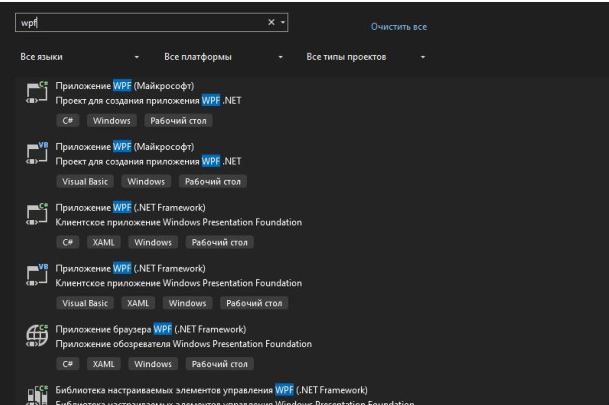
\includegraphics[width=0.6\textwidth]{fig/projectCreate.png}
		      \caption{Создание проекта}
		      \label{fig:projectcreate}
	      \end{figure}

	      % \item Далее задать имя проекта: StoreManager
	\item Далее задать имя проекта: StoreManager (Рисунок \ref{fig:createnameproject})

	      \begin{figure}[H]
		      \centering
		      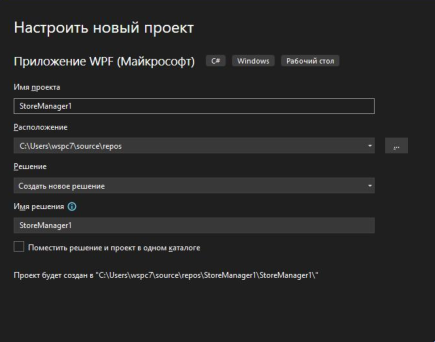
\includegraphics[width=0.6\textwidth]{fig/createNameProject.png}
		      \caption{Задание имени проекта}
		      \label{fig:createnameproject}
	      \end{figure}

	      \newpage

	      % \item Выбрать платформу (пример выполненн на .net 8.0)
	\item Выбрать платформу (пример выполненн на .net 8.0) (Рисунок \ref{fig:net8})

	      \begin{figure}[H]
		      \centering
		      
\includegraphics[width=0.8\textwidth]{fig/net8.0.png}
		      \caption{Задание имени проекта.}
		      \label{fig:net8}
	      \end{figure}

\end{enumerate}

Структура проекта состоит из следующих файлов:

\begin{itemize}
	\item App.xaml — конфигурация приложения. Определяет основной класс приложения, наследуемый от Application. В нём задаются стили, шаблоны приложения и стартовая точка\footnote{Обычно указывается начальное окно в свойстве StartupUri}.
	\item App.xaml.cs — логика приложения Содержит класс App, который может переопределять методы, такие как OnStartup, для настройки поведения при запуске, или обрабатывать события приложения.
	\item MainWindow.xaml — разметка и структура UI (интерфейса) главного окна.
	\item MainWindow.xaml.cs — логика и обработчики событий окна.
\end{itemize}



\newpage

\subsection{ШАГ 2: ДОБАВЛЕНИЕ ФАЙЛОВ}

\stepcounter{subsubsection}
\phantomsection
\addcontentsline{toc}{subsubsection}{\numberline{\thesubsubsection}СОЗДАНИЕ ПАПКИ MODELS}

Необходимо добавить следующие файлы и папки:
\begin{itemize}
	\item В корне проекта создать папку Models
	\item В папке Models добавить два новых файла классов: Product.cs и Order.cs.
\end{itemize}

\noindent Код для файла Order.cs приведен в листинге \ref{lst:OrderCs}

\begin{lstlisting}[style=csharp_catppuccin, label={lst:OrderCs}, caption=Класс \colorGIT{\href{https://github.com/WebMasterIT/Csharp_Labs/blob/ec375afd16c0647b337cf3d8a79c8bef904fc1be/3lab/StoreManager/Models/Order.cs\#L1-L27}{Order.cs}}]
namespace StoreManager.Models
{
    // Модель заказа, содержащая информацию о клиенте и товарах
    public class Order
    {
        // Уникальный идентификатор заказа
        public int Id { get; set; }

        // Список элементов заказа (товар + количество)
        public List<OrderItem> Items { get; set; }

        // Имя клиента
        public string CustomerName { get; set; }

        // Дата создания заказа
        public DateTime OrderDate { get; set; }

        // Общая сумма заказа, вычисляемая как сумма цен товаров умноженная на их количество
        public decimal TotalPrice => Items.Sum(item => item.Product.Price * item.Quantity);

        // Конструктор, инициализирующий пустой список товаров
        public Order()
        {
            Items = new List<OrderItem>();
        }
    }
}
\end{lstlisting}

Данный файл отвечает за создание нового объекта заказа. Может содержать уникальные поля не такие как в примере (в соответствии с вариантом).

% \newpage

\stepcounter{subsubsection}
\phantomsection
\addcontentsline{toc}{subsubsection}{\numberline{\thesubsubsection}КЛАССЫ: PRODUCT.CS, ORDER.CS, ORDERITEM.CS}

Также необходим класс позволяющий связать товар и его количество в заказе. Пример, созданного класса OrderItem и объявления его свойств приведен в листинге \ref{lst:OrderItem}

\begin{lstlisting}[style=csharp_catppuccin, caption=Класс \colorGIT{\href{https://github.com/WebMasterIT/Csharp_Labs/blob/ec375afd16c0647b337cf3d8a79c8bef904fc1be/3lab/StoreManager/Models/OrderItem.cs\#L1-L12}{OrderItem}}, label=lst:OrderItem]
namespace StoreManager.Models
{
    // Модель элемента заказа, связывающая товар и его количество
    public class OrderItem
    {
        // Ссылка на товар
        public Product Product { get; set; }

        // Количество единиц товара в заказе
        public int Quantity { get; set; }
    }
}
\end{lstlisting}

Также необходимо создать файл Product.cs. Данный файл отвечает за создание нововго объекта товараю Пример, класса Product приведен в листинге \ref{lst:Product.cs}.

\newpage

\begin{lstlisting}[style=csharp_catppuccin, caption=Класс \colorGIT{\href{https://github.com/WebMasterIT/Csharp_Labs/blob/ec375afd16c0647b337cf3d8a79c8bef904fc1be/3lab/StoreManager/Models/Product.cs\#L1-L18}{Product.cs}}, label=lst:Product.cs]
namespace StoreManager.Models
{
    {
    // Модель товара, представляющая продукт в магазине
    public class Product
    {
        // Уникальный идентификатор товара
        public int Id { get; set; }

        // Название товара
        public string Name { get; set; }

        // Цена товара
        public decimal Price { get; set; }

        // Количество товара на складе
        public int Stock { get; set; }
    }
}   
\end{lstlisting}

% \newpage

Также необходимо создать папку Converters. Она будет нужна для создания конвертера. В данной папке нужно создать класс BooleanToVisibilityConverter. Пример разметки для данного класса приведен в листинге \ref{lst:BooleanToVisibilityConverter}.
\begin{lstlisting}[style=csharp_catppuccin, caption=Класс \colorGIT{\href{https://github.com/WebMasterIT/Csharp_Labs/blob/ec375afd16c0647b337cf3d8a79c8bef904fc1be/3lab/StoreManager/Converters/BooleanToVisibilityConverter.cs\#L1-L23}{BooleanToVisibilityConverter}}, label=lst:BooleanToVisibilityConverter]
using System;
using System.Globalization;
using System.Windows;
using System.Windows.Data;

namespace StoreManager.Converters
{
    // Конвертер для отображения placeholder'ов в TextBox
    public class BooleanToVisibilityConverter : IValueConverter
    {
        // Преобразует boolean (IsEmpty) в Visibility для TextBlock
        public object Convert(object value, Type targetType, object parameter, CultureInfo culture)
        {
            return value is bool isEmpty && isEmpty ? Visibility.Visible : Visibility.Collapsed;
        }

        // Обратное преобразование не используется
        public object ConvertBack(object value, Type targetType, object parameter, CultureInfo culture)
        {
            throw new NotImplementedException();
        }
    }
}
\end{lstlisting}

Этот класс реализует интерфейс IValueConverter, который используется для
преобразования данных при привязке (Data Binding)
\begin{itemize}
	\item Метод Convert преобразует значение типа bool в Visibility (перечисление WPF для управления видимостью элементов)
	\item true \icon{} Visibility.Visible (элемент виден)
	\item false \icon{} Visibility.Collapsed (элемент скрыт, не занимает место
	\item Метод ConvertBack не реализован, так как обратное преобразование не требуется.
\end{itemize}

\newpage
Конвертеры в WPF используются для преобразования данных между источником
(моделью) и целью (элементом UI). Например, конвертер позволяет адаптировать
значение свойства модели к формату, подходящему для отображения. В данном
случае конвертер применяется для реализации эффекта placeholder (подсказки в
текстовых полях), показывая текст, когда поле пустое (Text.IsEmpty).

Свойство Visibility в WPF имеет три значения
\begin{itemize}
	\item Visible -- элемент отображается
	\item Collapsed -- элемент скрыт и не занимает места
	\item Hidden -- элемент скрыт, но занимает место в макете.
\end{itemize}

\subsection{ШАГ 3: РЕАЛИЗАЦИЯ ИНТЕРФЕЙСА}

Для того чтобы реализовать внешний вид приложения необходимо добавить
соответствующую разметку в файл MainWindow.xaml
Пример разметки для данного файла будет представлен ниже в листинге \ref{lst:MainWindow}

% TODO:
% 1. покрасить код
% 2. спросить, что делать с эти листингом, мб тпропнуть его?

\begin{lstlisting}[style=csharp_catppuccin, caption=Пример разметки главного окна \colorGIT{\href{https://github.com/WebMasterIT/Csharp_Labs/blob/ec375afd16c0647b337cf3d8a79c8bef904fc1be/3lab/StoreManager/MainWindow.xaml\#L1-L200}{MainWindow}}, label=lst:MainWindow, basicstyle=\tiny]
<Window x:Class="StoreManager.MainWindow"
        xmlns="http://schemas.microsoft.com/winfx/2006/xaml/presentation"
        xmlns:x="http://schemas.microsoft.com/winfx/2006/xaml"
        xmlns:converters="clr-namespace:StoreManager.Converters"
        Title="Управление магазином" Height="650" Width="950"
        WindowStartupLocation="CenterScreen" Background="#F5F5F5">

    <!-- Ресурсы окна: конвертеры и стили -->
    <Window.Resources>
        <!-- Конвертер для преобразования bool в Visibility -->
        <converters:BooleanToVisibilityConverter x:Key="BooleanToVisibilityConverter"/>

        <!-- Общий стиль кнопок -->
        <Style TargetType="Button">
            <Setter Property="Background" Value="#FF6200EE"/>
            <Setter Property="Foreground" Value="White"/>
            <Setter Property="FontSize" Value="14"/>
            <Setter Property="Padding" Value="10,5"/>
            <Setter Property="Margin" Value="5"/>
            <Setter Property="BorderThickness" Value="0"/>
            <Setter Property="Cursor" Value="Hand"/>
        </Style>

        <!-- Специальный стиль кнопок изменения количества -->
        <Style x:Key="QuantityButtonStyle" TargetType="Button">
            <Setter Property="Background" Value="#FF6200EE"/>
            <Setter Property="Foreground" Value="White"/>
            <Setter Property="FontSize" Value="12"/>
            <Setter Property="Width" Value="25"/>
            <Setter Property="Height" Value="25"/>
            <Setter Property="Margin" Value="5,0"/>
            <Setter Property="BorderThickness" Value="0"/>
            <Setter Property="Cursor" Value="Hand"/>
        </Style>

        <!-- Стиль для полей ввода -->
        <Style TargetType="TextBox">
            <Setter Property="FontSize" Value="14"/>
            <Setter Property="Padding" Value="5"/>
            <Setter Property="Margin" Value="5"/>
            <Setter Property="BorderBrush" Value="#FFCCCCCC"/>
        </Style>

        <!-- Стиль текста-заглушки (placeholder) -->
        <Style TargetType="TextBlock" x:Key="PlaceholderStyle">
            <Setter Property="Foreground" Value="Gray"/>
            <Setter Property="FontStyle" Value="Italic"/>
            <Setter Property="Margin" Value="8,5,0,0"/>
            <Setter Property="IsHitTestVisible" Value="False"/>
        </Style>
    </Window.Resources>

    <!-- Основная сетка, задаёт структуру окна -->
    <Grid Margin="-16,0,0,-35">
        <Grid.ColumnDefinitions>
            <!-- Колонки для панели товаров и заказов -->
            <ColumnDefinition Width="107*"/>
            <ColumnDefinition Width="344*"/>
            <ColumnDefinition Width="450*"/>
        </Grid.ColumnDefinitions>

        <!-- Панель товаров -->
        <Border Grid.Column="0" Margin="10" Background="White" CornerRadius="10" Padding="10" Grid.ColumnSpan="2">
            <StackPanel>
                <TextBlock Text="Товары" FontSize="20" FontWeight="Bold" Margin="0,0,0,10"/>

                <!-- Список товаров -->
                <ListBox x:Name="ProductsList" Height="250" BorderBrush="#FFCCCCCC" 
                         SelectionChanged="ProductsList_SelectionChanged" 
                         MouseLeftButtonDown="ProductsList_MouseLeftButtonDown">
                    <ListBox.ItemTemplate>
                        <DataTemplate>
                            <StackPanel Orientation="Horizontal">
                                <!-- Название -->
                                <TextBlock Text="{Binding Name}" FontWeight="Bold" Margin="0,0,10,0"/>
                                <!-- Цена -->
                                <TextBlock Text="{Binding Price, StringFormat={}{0:C}}"/>
                                <!-- Остаток -->
                                <TextBlock Text=" (Остаток: " FontStyle="Italic"/>
                                <TextBlock Text="{Binding Stock}">
                                    <!-- Подсветка остатка -->
                                    <TextBlock.Style>
                                        <Style TargetType="TextBlock">
                                            <Style.Triggers>
                                                <!-- Если 0 - красным -->
                                                <DataTrigger Binding="{Binding Stock}" Value="0">
                                                    <Setter Property="Foreground" Value="Red"/>
                                                </DataTrigger>
                                                <!-- Если меньше 5 - оранжевым -->
                                                <DataTrigger Binding="{Binding Stock, ConverterParameter=5}" Value="True">
                                                    <Setter Property="Foreground" Value="Orange"/>
                                                </DataTrigger>
                                            </Style.Triggers>
                                        </Style>
                                    </TextBlock.Style>
                                </TextBlock>
                                <TextBlock Text=")"/>
                            </StackPanel>
                        </DataTemplate>
                    </ListBox.ItemTemplate>
                </ListBox>

                <!-- Кнопка добавления в заказ -->
                <Button x:Name="AddToOrderButton" Content="Добавить в заказ" Click="AddToOrder_Click" HorizontalAlignment="Right"/>

                <!-- Поля ввода нового товара -->
                <Grid>
                    <TextBox x:Name="ProductName"/>
                    <TextBlock Text="Название товара" Style="{StaticResource PlaceholderStyle}"
                               Visibility="{Binding ElementName=ProductName, Path=Text.IsEmpty, Converter={StaticResource BooleanToVisibilityConverter}}"/>
                </Grid>
                <Grid>
                    <TextBox x:Name="ProductPrice"/>
                    <TextBlock Text="Цена" Style="{StaticResource PlaceholderStyle}"
                               Visibility="{Binding ElementName=ProductPrice, Path=Text.IsEmpty, Converter={StaticResource BooleanToVisibilityConverter}}"/>
                </Grid>
                <Grid>
                    <TextBox x:Name="ProductStock"/>
                    <TextBlock Text="Остаток" Style="{StaticResource PlaceholderStyle}"
                               Visibility="{Binding ElementName=ProductStock, Path=Text.IsEmpty, Converter={StaticResource BooleanToVisibilityConverter}}"/>
                </Grid>

                <!-- Кнопки управления товарами -->
                <StackPanel HorizontalAlignment="Right" Width="222">
                    <Button Content="Добавить товар" Click="AddProduct_Click"/>
                    <Button Content="Обновить товар" Click="UpdateProduct_Click"/>
                    <Button Content="Удалить товар" Click="DeleteProduct_Click"/>
                </StackPanel>
            </StackPanel>
        </Border>

        <!-- Панель заказов -->
        <Border Grid.Column="2" Margin="10" Background="White" CornerRadius="10" Padding="10">
            <StackPanel>
                <TextBlock Text="Заказы" FontSize="20" FontWeight="Bold" Margin="0,0,0,10"/>

                <!-- Список заказов -->
                <ListBox x:Name="OrdersList" Height="150" BorderBrush="#FFCCCCCC"
                         SelectionChanged="OrdersList_SelectionChanged"
                         MouseLeftButtonDown="ProductsList_MouseLeftButtonDown">
                    <ListBox.ItemTemplate>
                        <DataTemplate>
                            <StackPanel>
                                <TextBlock Text="{Binding CustomerName}" FontWeight="Bold"/>
                                <TextBlock Text="{Binding OrderDate, StringFormat={}{0:dd.MM.yyyy HH:mm}}"/>
                                <TextBlock Text="{Binding TotalPrice, StringFormat=Итого: {0:C}}"/>
                                <!-- Список товаров в заказе -->
                                <ItemsControl ItemsSource="{Binding Items}">
                                    <ItemsControl.ItemTemplate>
                                        <DataTemplate>
                                            <StackPanel Orientation="Horizontal">
                                                <TextBlock Text="{Binding Product.Name}" Margin="0,0,10,0"/>
                                                <TextBlock Text="{Binding Product.Price, StringFormat={}{0:C}}"/>
                                                <TextBlock Text=" x " FontStyle="Italic"/>
                                                <TextBlock Text="{Binding Quantity}"/>
                                            </StackPanel>
                                        </DataTemplate>
                                    </ItemsControl.ItemTemplate>
                                </ItemsControl>
                            </StackPanel>
                        </DataTemplate>
                    </ListBox.ItemTemplate>
                </ListBox>

                <!-- Список выбранных товаров для нового заказа -->
                <TextBlock Text="Выбранные товары для заказа" FontSize="14" FontWeight="Bold" Margin="0,10,0,5"/>
                <ListBox x:Name="SelectedProductsList" Height="100" BorderBrush="#FFCCCCCC" MouseLeftButtonDown="ProductsList_MouseLeftButtonDown">
                    <ListBox.ItemTemplate>
                        <DataTemplate>
                            <StackPanel Orientation="Horizontal">
                                <TextBlock Text="{Binding Product.Name}" FontWeight="Bold" Margin="0,0,10,0"/>
                                <TextBlock Text="{Binding Product.Price, StringFormat={}{0:C}}"/>
                                <TextBlock Text=" x " FontStyle="Italic"/>
                                <TextBlock Text="{Binding Quantity}" Margin="0,0,10,0"/>
                                <!-- Кнопки изменения количества -->
                                <Button Content="+" Style="{StaticResource QuantityButtonStyle}" Click="IncreaseQuantity_Click" Tag="{Binding}"/>
                                <Button Content="-" Style="{StaticResource QuantityButtonStyle}" Click="DecreaseQuantity_Click" Tag="{Binding}"/>
                            </StackPanel>
                        </DataTemplate>
                    </ListBox.ItemTemplate>
                </ListBox>

                <!-- Кнопка удаления товара из заказа -->
                <Button Content="Удалить товар из заказа" Click="RemoveProductFromOrder_Click" HorizontalAlignment="Right"/>

                <!-- Поле ввода имени клиента -->
                <Grid>
                    <TextBox x:Name="CustomerName"/>
                    <TextBlock Text="Имя клиента" Style="{StaticResource PlaceholderStyle}"
                               Visibility="{Binding ElementName=CustomerName, Path=Text.IsEmpty, Converter={StaticResource BooleanToVisibilityConverter}}"/>
                </Grid>

                <!-- Кнопки управления заказами -->
                <StackPanel Orientation="Horizontal" HorizontalAlignment="Right">
                    <Button Content="Создать заказ" Click="AddOrder_Click"/>
                    <Button Content="Обновить заказ" Click="UpdateOrder_Click"/>
                    <Button Content="Удалить заказ" Click="DeleteOrder_Click"/>
                </StackPanel>
            </StackPanel>
        </Border>
    </Grid>
</Window>
\end{lstlisting}

\newpage

\subsection{ШАГ 4: РЕАЛИЗАЦИЯ ЛОГИКИ}

Файл MainWindow.xaml.cs -- это code-behind для главного окна приложения. Он содержит логику взаимодействия пользовательского интерфейса (UI) с данными, обрабатывает события (например, нажатия кнопок) и управляет состоянием приложения. Приложение представляет собой систему управления магазином, где пользователь может.

Структура кода состоит из следующих элементов
\begin{enumerate}
	\item Объявления класса и полей -- определение данных, используемых в приложении
	\item Конструктора -- инициализация окна и начальных данных
	\item Методов обновления UI -- синхронизация списков товаров и заказов с UI
	\item Обработчиков событий -- реакция на действия пользователя (нажатия кнопок, выбор элементов)
	\item Вспомогательных методов -- очистка полей ввода.
\end{enumerate}
В листинге \ref{lst:Main} представлен пример кода для класса MainWindow.

\begin{lstlisting}[style=csharp_catppuccin, caption=Пример кода для класса \colorGIT{\href{https://github.com/WebMasterIT/Csharp_Labs/blob/ec375afd16c0647b337cf3d8a79c8bef904fc1be/3lab/StoreManager/MainWindow.xaml.cs\#L1-L21}{Main}}, label=lst:Main]
using StoreManager.Models;
using System.Windows;
using System.Windows.Controls;
using System.Windows.Input;
using System.Windows.Media;

namespace StoreManager
{
    // Главное окно приложения для управления товарами и заказами
    public partial class MainWindow : Window
    {
        // Список всех товаров
        private List<Product> products = new List<Product>();
        // Список всех заказов
        private List<Order> orders = new List<Order>();
        // Следующий ID для нового товара
        private int nextProductId = 1;
        // Следующий ID для нового заказа
        private int nextOrderId = 1;
        // Список выбранных товаров для текущего заказа
        private List<OrderItem> selectedProductsForOrder = new List<OrderItem>();
\end{lstlisting}

Класс MainWindow наследуется от Window, так как это главное окно WPF-приложения. Ключевое слово partial указывает, что класс разделён между MainWindow.xaml.cs (логика) и MainWindow\-.xaml (разметка, сгенерированная часть).

Поля:
\begin{itemize}
	\item products: Хранит список всех товаров (экземпляры класса Product). Это основная коллекция для управления ассортиментом магазина
	\item orders: Хранит список заказов (экземпляры класса Order). Каждый заказ содержит имя клиента, дату и список товаров
	\item nextProductId: Счётчик для генерации уникальных идентификаторов товаров.
\end{itemize}

\pagebreak

Начинается с 1 и увеличивается при добавлении нового товара
\begin{itemize}
	\item nextOrderId: Аналогичный счётчик для заказов
	\item selectedProductsForOrder: Временное хранилище товаров (OrderItem), которые пользователь выбрал при формировании нового заказа.
\end{itemize}

Эти поля представляют состояние приложения. Они хранят данные в памяти (вместо базы данных) и используются для отображения в UI и обработки пользовательских действий. Использование List<T> означает, что данные не обновляют UI автоматически (в отличие от ObservableCollection), поэтому код вручную обновляет списки. Далее необходимо объявить основной метод MainWindow.
Пример кода для данного метода представлен в листинге \ref{lst:Main2}

\begin{lstlisting}[style=csharp_catppuccin, caption=Пример кода для класса \colorGIT{\href{https://github.com/WebMasterIT/Csharp_Labs/blob/ec375afd16c0647b337cf3d8a79c8bef904fc1be/3lab/StoreManager/MainWindow.xaml.cs\#L24-L30}{Main}}, label=lst:Main2]
        public MainWindow()
        {
            InitializeComponent(); // Инициализация UI
            UpdateProductList();   // Обновление списка товаров
            UpdateOrderList();    // Обновление списка заказов
            UpdateSelectedProductsList(); // Обновление списка выбранных товаров
        }
\end{lstlisting}

InitializeComponent() — метод, автоматически сгенерированный WPF, который загружает разметку из MainWindow.xaml, инициализирует элементы интерфейса (такие как кнопки, списки и текстовые поля) и устанавливает необходимые привязки. Без его вызова пользовательский интерфейс не будет отображён.

Вызовы методов обновления:
\begin{itemize}
	\item UpdateProductList() — устанавливает ItemsSource для ListBox с товарами, чтобы отобразить начальный список (пустой на старте)
	\item UpdateOrderList() — аналогично предыдущему методу, только для списка заказов (OrdersList)
	\item UpdateSelectedProductsList() -- обновляет список выбранных товаров для заказа (Selected\-Products\-List).
\end{itemize}

Назначение:
\begin{itemize}
	\item Конструктор подготавливает приложение к работе, загружая UI и синхронизируя данные с элементами управления
	\item Поскольку списки изначально пусты, вызовы обновления предотвращают ошибки отображения.
\end{itemize}

\pagebreak

Методы для обновления списков товаров, заказов и выбранных товаров для заказа
представлены в листинге \ref{lst:Method}


\begin{lstlisting}[style=csharp_catppuccin, caption=\colorGIT{\href{https://github.com/WebMasterIT/Csharp_Labs/blob/ec375afd16c0647b337cf3d8a79c8bef904fc1be/3lab/StoreManager/MainWindow.xaml.cs\#L32-L51}{Методы}} обновления данных, label=lst:Method]
        // Обновляет отображение списка товаров
        private void UpdateProductList()
        {
            ProductsList.ItemsSource = null;
            ProductsList.ItemsSource = products;
        }

        // Обновляет отображение списка заказов
        private void UpdateOrderList()
        {
            OrdersList.ItemsSource = null;
            OrdersList.ItemsSource = orders;
        }

        // Обновляет отображение списка выбранных товаров
        private void UpdateSelectedProductsList()
        {
            SelectedProductsList.ItemsSource = null;
            SelectedProductsList.ItemsSource = selectedProductsForOrder;
        }
\end{lstlisting}

Метод UpdateProductList Сбрасывает ItemsSource в null, чтобы очистить привязку. Устанавливает ItemsSource в products, чтобы ListBox (ProductsList) отобразил текущий список товаров. Остальные методы работают аналогично. Null используется для предотвращения проблемы с кэшированием данных в WPF, обеспечивая корректное обновление интерфейса.

\newpage

Далее рассмотрим методы для работы с конкретными товарами. Эти методы реагируют на действия пользователя с товарами (кнопки «Добавить», «Обновить», «Удалить», выбор в списке). Метод добавления нового товара представлен в листинге \ref{lst:MethodAdd}
\begin{lstlisting}[style=csharp_catppuccin, caption=\colorGIT{\href{https://github.com/WebMasterIT/Csharp_Labs/blob/ec375afd16c0647b337cf3d8a79c8bef904fc1be/3lab/StoreManager/MainWindow.xaml.cs\#L53-L80}{Метод}} добавления нового товара, label=lst:MethodAdd]
        // Обработчик нажатия кнопки "Добавить товар"
        private void AddProduct_Click(object sender, RoutedEventArgs e)
        {
            // Проверка корректности введённых данных
            if (string.IsNullOrWhiteSpace(ProductName.Text) ||
                !decimal.TryParse(ProductPrice.Text, out decimal price) ||
                !int.TryParse(ProductStock.Text, out int stock) ||
                stock < 0)
            {
                MessageBox.Show(
                    """
                    Пожалуйста, введите корректные данные о товаре.
                    Остаток не может быть отрицательным.
                    """
                    "Ошибка",
                    MessageBoxButton.OK,
                    MessageBoxImage.Error
                );

                return;
            }

            // Создание нового товара
            var product = new Product
            {
                Id = nextProductId++,
                Name = ProductName.Text,
                Price = price,
                Stock = stock
            };

            products.Add(product); // Добавление товара в список
            UpdateProductList();    // Обновление UI
            ClearProductFields();   // Очистка полей ввода
        }
\end{lstlisting}

Данный метод проверяет валидность ввода:
\begin{itemize}
	\item productName.Text не пустое.
	\item проверка productPrice.Text (что цена корректна (decimal), количество -- неотрицательное число).
	\item productStock.Text преобразуется в int.
\end{itemize}

Если валидация не пройдена, показывает сообщение об ошибке. Создаёт новый объект Product с уникальным Id (из nextProductId), именем, ценой и запасом из полей ввода. Далее добавляет товар в список products, обновляет UI (UpdateProductList) и очищает поля ввода (ClearProductFields).

\newpage

Следующий метод позволяет обновить (редактировать) информацию о конкретном товаре. Реализация метода обновления представлен в листинге \ref{lst:MethodUpdate}

\begin{lstlisting}[style=csharp_catppuccin, caption=\colorGIT{\href{https://github.com/WebMasterIT/Csharp_Labs/blob/ec375afd16c0647b337cf3d8a79c8bef904fc1be/3lab/StoreManager/MainWindow.xaml.cs\#L82-L110}{Метод}} обновления нового товара, label=lst:MethodUpdate]
        // Обработчик нажатия кнопки "Обновить товар"
        private void UpdateProduct_Click(object sender, RoutedEventArgs e)
        {
            if (ProductsList.SelectedItem is Product selectedProduct)
            {
                // Проверка корректности введённых данных
                if (string.IsNullOrWhiteSpace(ProductName.Text) ||
                    !decimal.TryParse(ProductPrice.Text, out decimal price) ||
                    !int.TryParse(ProductStock.Text, out int stock) ||
                    stock < 0)
                {
                    MessageBox.Show(
                        "Пожалуйста, введите корректные данные о товаре. " +
                        "Остаток не может быть отрицательным.",
                        "Ошибка",
                        MessageBoxButton.OK,
                        MessageBoxImage.Error
                    );
                        "Ошибка", MessageBoxButton.OK, MessageBoxImage.Error);
                    return;
                }

                // Обновление свойств выбранного товара
                selectedProduct.Name = ProductName.Text;
                selectedProduct.Price = price;
                selectedProduct.Stock = stock;

                UpdateProductList();  // Обновление UI
                ClearProductFields(); // Очистка полей ввода
            }
            else
            {
                MessageBox.Show(
                    "Пожалуйста, выберите товар для обновления.",
                    "Ошибка",
                    MessageBoxButton.OK,
                    MessageBoxImage.Warning
                );
            }
        }
\end{lstlisting}


Данный метод проверяет, выбран ли товар в списке ProductsList.
\begin{itemize}
	\item проводит валидацию ввода (аналогично AddProduct\_Click)
	\item если товар выбран и данные валидны, обновляет свойства выбранного объекта Product (Name, Price, Stock)
	\item обновляет UI и очищает поля
	\item если товар не выбран, показывает предупреждение.
\end{itemize}

\newpage

\section{ШАГ 5: ВНЕШНИЙ ВИД ИНТЕРФЕЙСА \ \texorpdfstring{\faBrush}{}}
\section{ШАГ 6: ДЕМОНСТРАЦИЯ РАБОТЫ \ \texorpdfstring{\faGlasses}{}}

\newpage

\section{ВОПРОСЫ ДЛЯ ЗАЩИТЫ~\texorpdfstring{\icon{}}{}}
\begin{enumerate}
	\item вопрос
	\item вопрос
	\item вопрос
	\item вопрос
	\item вопрос
	\item вопрос
	\item вопрос
	\item вопрос
	\item вопрос
	\item вопрос
\end{enumerate}

\lipsum[4-7]

\end{document}
